\section{Proton-Proton collisions at the LHC}
\subsection{An Introduction to Particle Accelerators and Detecors}
With a circumference of 27 km, the \emph{particle accelerator} \ac{LHC} is the largest piece of scientific 
equipment ever built. It consists of two separate large tubes aligned with powerful magnets. The magnets are used 
to accelerate bunches\footnote{Small pockets of particles} of hadrons (specifically protons) and lead. One set 
of bunches are accelerated in one of the tubes, and another set is accelerated in the other direction inside the 
other tube. The bunches are accelerated up to close (v=0.99999991c) the speed of light before they collide at a 
rate of once every 25 nanosecond. The released energy from the collisions enable the creations of new particles.
\\
To measure the collisions, we use \emph{particle detectors}. In this thesis I will be using data collected by the 
\acs{ATLAS} (\acl{ATLAS}) detector. The \ac{ATLAS}-detector is the largest general-purpose detector at the \ac{LHC}
and was first active in 2009. The detector consists of several ever-increasing cylindrical layers around the point of 
collision. In figure \ref{fig:detector}, taken from the \ac{ATLAS} collaboration \cite{PDetector} the cross section 
of the detector along with the paths of different particles is visualized. The inside of a detector can be summarized 
in the following points, listed from innermost to outermost layer:
\begin{itemize}
    \item \emph{Inner Detector}: The inner detector consists of three layers, Pixel detector, Semi-Conductor Tracker 
          and Transition Radiation Tracker. Its purpose is to measure electromagnetic interactions between the particles 
          produced in the collision and the material in the layers. The measurements are made at discrete points and can be 
          used to infer the momentum of the particles. An electromagnetic field is applied to the inner detector
          to curve the paths of the particles, so to measure properties of the particles like spin and charge.  
    \item \emph{Calorimeters}: The ATLAS detector has two calorimeters, the \emph{Electromagnetic calorimeter} and the 
           \emph{Hadronic calorimeter}. The \ac{EM} calorimeter is the first layer of the two and measures the energy of 
           particles interacting through the \ac{EM} field. The hadronic calorimeter is designed to measure the energy of 
           hadrons (i.e. protons, neutrons, mesons etc.).
    \item \emph{Muon Spectrometer}: The muon spectrometer is included to detect muons, which would otherwise not be measured 
           by the previous layers. Similarly to the inner detector, the muon spectrometer applies a \ac{EM} field to 
           curve the path of the particles which allows it to measure several properties. 
\end{itemize}
\begin{figure}
    \centering
    \makebox[0.75\linewidth][c]{%
    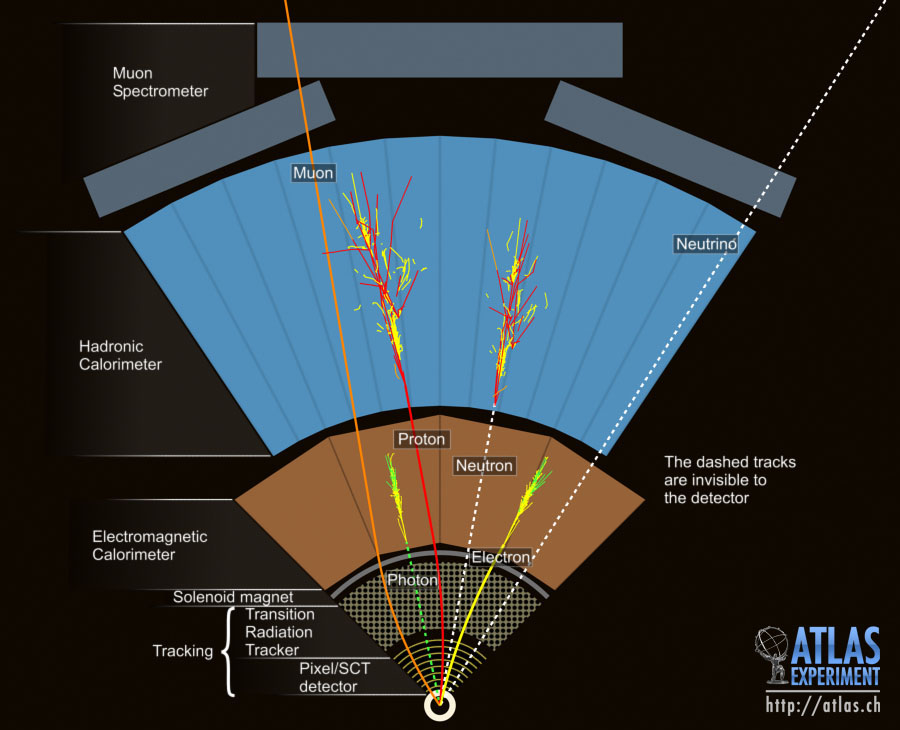
\includegraphics[width=0.75\textwidth]{Figures/Illustrations/detector.jpeg}
    }
    \caption{Event Cross Section in a computer generated image of the
    ATLAS detector \cite{PDetector}.}
    \label{fig:detector}
\end{figure}

\subsection{The Kinematics}